\begin{figure}[h!]
   \centering
   \begin{subfigure}[b]{0.4\textwidth}
      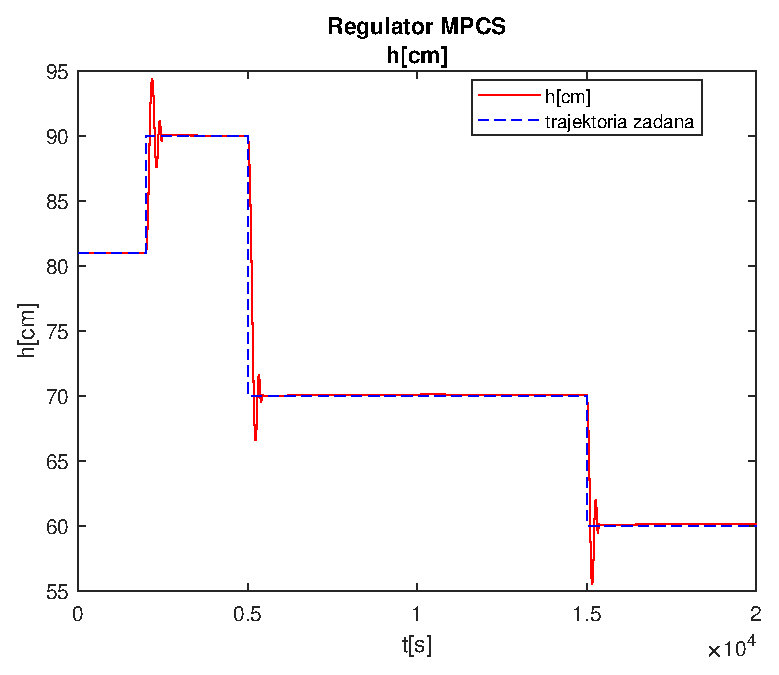
\includegraphics[width=1\linewidth]{img/MPCSanaRK/MPCSRKHN100Nu10l10.eps}
      \caption{}
      \label{fig:fig:MPCSRKN100Nu10l101}
   \end{subfigure}
       
   \begin{subfigure}[b]{0.4\textwidth}
      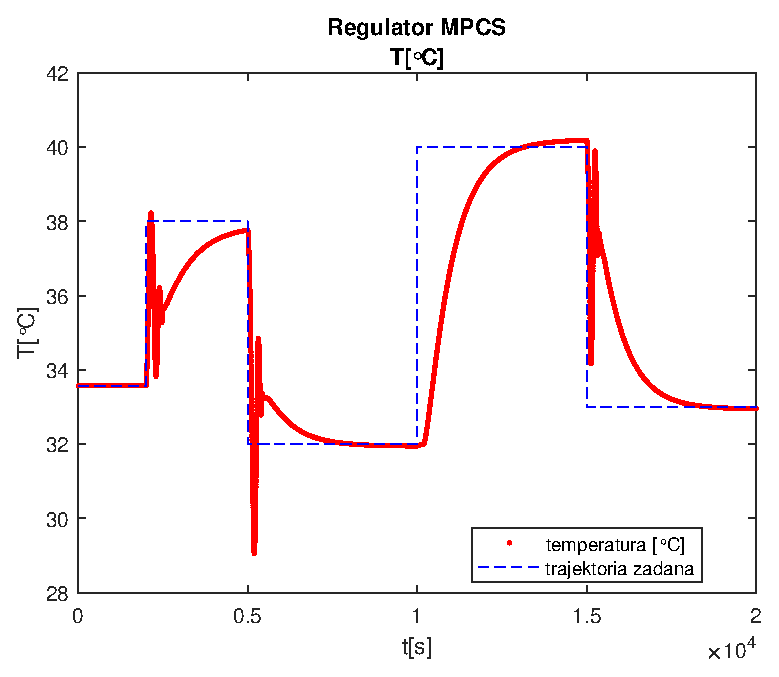
\includegraphics[width=1\linewidth]{img/MPCSanaRK/MPCSRKTN100Nu10l10.eps}
      \caption{}
      \label{fig:fig:MPCSRKN100Nu10l102}
   \end{subfigure}
       
   \begin{subfigure}[b]{0.4\textwidth}
      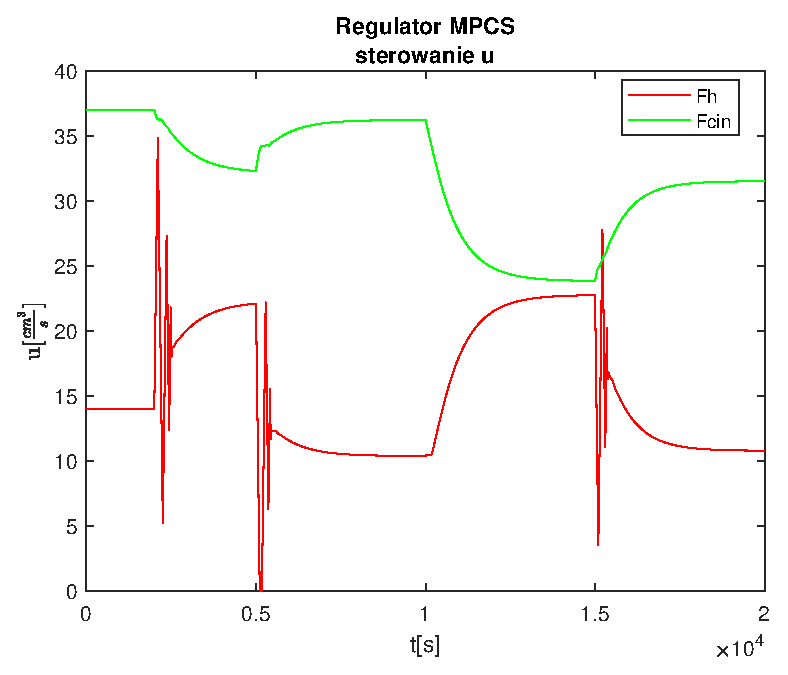
\includegraphics[width=1\linewidth]{img/MPCSanaRK/MPCSRKControlN100Nu10l10.eps}
      \caption{}
      \label{fig:fig:MPCSRKN100Nu10l103}
   \end{subfigure}
       
   \caption{Wykresy dla regulatora MPCS, obiekt nieliniowy.}
   \label{fig:MPCSRKN100Nu10l10}
\end{figure}
           
